% Iterator class inheritance hierarchy — vertical tree layout
\documentclass[tikz,border=3mm]{standalone}
\usepackage[T1]{fontenc}
\usepackage{lmodern}
\usetikzlibrary{arrows.meta}

\begin{document}
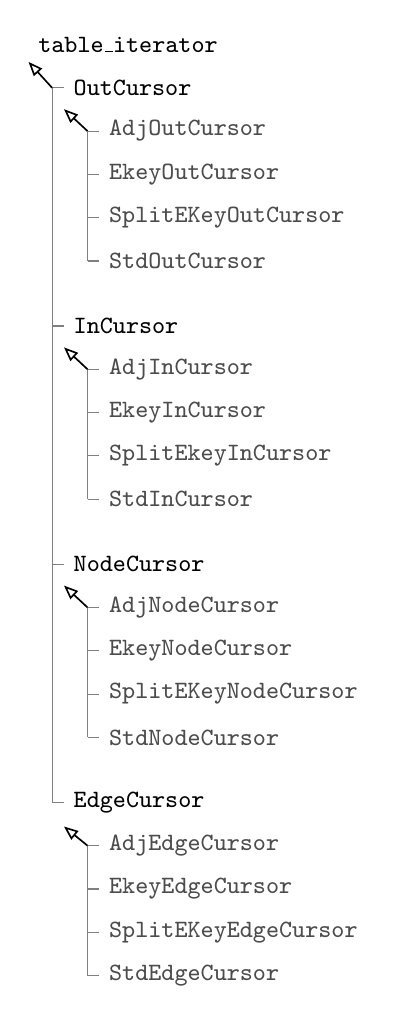
\begin{tikzpicture}[
  base/.style={font=\small\ttfamily\bfseries},
  abst/.style={font=\small\ttfamily},
  impl/.style={font=\small\ttfamily, text=black!70},
  every node/.style={anchor=west},
  inh/.style={-{Triangle[open,length=1.8mm,width=1.4mm]}, semithick},
  ext/.style={-, thin, black!50},
]

\def\LV{5.5mm}   % line vertical spacing
\def\I{4.5mm}    % indent per level

% Root
\node[base] (root) at (0,0) {table\_iterator};

% ── OutCursor subtree ──
\node[abst] (out) at (\I, -\LV) {OutCursor};
\node[impl] (a1) at (2*\I, -2*\LV) {AdjOutCursor};
\node[impl] (a2) at (2*\I, -3*\LV) {EkeyOutCursor};
\node[impl] (a3) at (2*\I, -4*\LV) {SplitEKeyOutCursor};
\node[impl] (a4) at (2*\I, -5*\LV) {StdOutCursor};

% ── InCursor subtree ──
\node[abst] (inc) at (\I, -6.5*\LV) {InCursor};
\node[impl] (b1) at (2*\I, -7.5*\LV) {AdjInCursor};
\node[impl] (b2) at (2*\I, -8.5*\LV) {EkeyInCursor};
\node[impl] (b3) at (2*\I, -9.5*\LV) {SplitEkeyInCursor};
\node[impl] (b4) at (2*\I, -10.5*\LV) {StdInCursor};

% ── NodeCursor subtree ──
\node[abst] (nod) at (\I, -12*\LV) {NodeCursor};
\node[impl] (c1) at (2*\I, -13*\LV) {AdjNodeCursor};
\node[impl] (c2) at (2*\I, -14*\LV) {EkeyNodeCursor};
\node[impl] (c3) at (2*\I, -15*\LV) {SplitEKeyNodeCursor};
\node[impl] (c4) at (2*\I, -16*\LV) {StdNodeCursor};

% ── EdgeCursor subtree ──
\node[abst] (edg) at (\I, -17.5*\LV) {EdgeCursor};
\node[impl] (d1) at (2*\I, -18.5*\LV) {AdjEdgeCursor};
\node[impl] (d2) at (2*\I, -19.5*\LV) {EkeyEdgeCursor};
\node[impl] (d3) at (2*\I, -20.5*\LV) {SplitEKeyEdgeCursor};
\node[impl] (d4) at (2*\I, -21.5*\LV) {StdEdgeCursor};

% ── Tree lines: root -> abstract cursors ──
% Vertical trunk from root
\draw[ext] ([xshift=-1.5mm]out.west) -- ([xshift=-1.5mm]edg.west);
\foreach \n in {out,inc,nod,edg}
  \draw[ext] ([xshift=-1.5mm]\n.west) -- (\n.west);

% Trunk anchor to root
\draw[inh] ([xshift=-1.5mm]out.west) -- (root.south west);

% ── Tree lines: abstract -> concrete ──
% OutCursor children
\draw[ext] ([xshift=-1.5mm]a1.west) -- ([xshift=-1.5mm]a4.west);
\foreach \n in {a1,a2,a3,a4}
  \draw[ext] ([xshift=-1.5mm]\n.west) -- (\n.west);
\draw[inh] ([xshift=-1.5mm]a1.west) -- ([yshift=-0.5mm]out.south west);

% InCursor children
\draw[ext] ([xshift=-1.5mm]b1.west) -- ([xshift=-1.5mm]b4.west);
\foreach \n in {b1,b2,b3,b4}
  \draw[ext] ([xshift=-1.5mm]\n.west) -- (\n.west);
\draw[inh] ([xshift=-1.5mm]b1.west) -- ([yshift=-0.5mm]inc.south west);

% NodeCursor children
\draw[ext] ([xshift=-1.5mm]c1.west) -- ([xshift=-1.5mm]c4.west);
\foreach \n in {c1,c2,c3,c4}
  \draw[ext] ([xshift=-1.5mm]\n.west) -- (\n.west);
\draw[inh] ([xshift=-1.5mm]c1.west) -- ([yshift=-0.5mm]nod.south west);

% EdgeCursor children
\draw[ext] ([xshift=-1.5mm]d1.west) -- ([xshift=-1.5mm]d4.west);
\foreach \n in {d1,d2,d3,d4}
  \draw[ext] ([xshift=-1.5mm]\n.west) -- (\n.west);
\draw[inh] ([xshift=-1.5mm]d1.west) -- ([yshift=-0.5mm]edg.south west);

\end{tikzpicture}
\end{document}
